\lecture{7}{Derivation of the Diffusion Equation}{2025-10-26}
\pagelayout{margin}
% --- Start writing here ---
\section*{Derivation of diffusion quation}
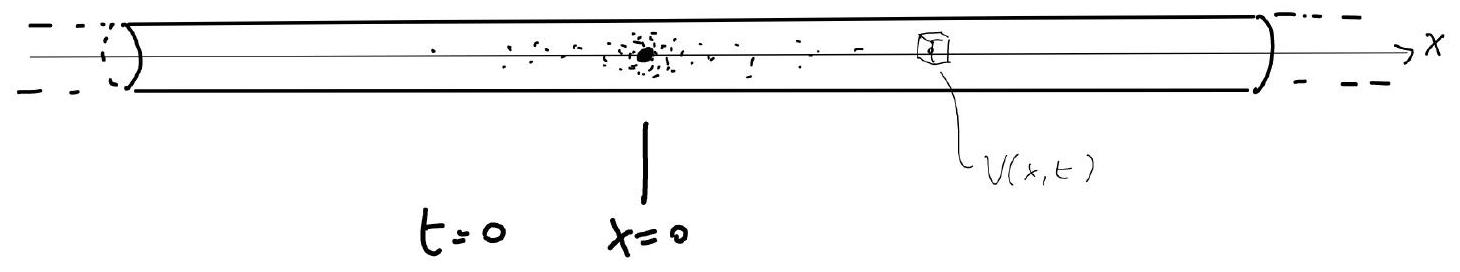
\includegraphics[width=\textwidth]{2025_10_26_8223bcdd8e86df21a973g-1}
\begin{DispWithArrows}[format=c, displaystyle]
w(x, t)=\lim _{\substack{V(x) \rightarrow 0 \ N \rightarrow \infty}} \frac{\text { \# of particles in } V(x, t)}{V(x, t)}
\end{DispWithArrows}
$W(x, t)$ is the density of Brownion particle at position $x$ and time $t \geqslant 0 . \quad W(x, t)$ is smooth and integrable:
\begin{DispWithArrows}[format=c, displaystyle]
\begin{aligned}
& \int_{-\infty}^{+\infty} w(x, t) d x=1 \\
& W(x, 0)=\delta(x)
\end{aligned}
\end{DispWithArrows}
$\int_{A} w(x, t) d x=$ prob. to find a Brownion porticle in the region $A \subseteq \mathbb{R}$ at any fine $t$.

Let's assume that the probability density that ar Brownion particle moves/jumps from $x$ to $x+y$ in a suall time interval $\Delta t$ is $f(y \mid x, \Delta t)=f(y, \Delta t)$ (notice that $f$ does not depend on $x$, though this is not a problem in general). Also, $\int_{-\infty}^{+\infty} f(y, \Delta t) d y=1$

We know $W(x, t)$ and $f(y, \Delta t)$, we want to desive the distribution of posticle at $x$ at fine $t+\Delta t$.

Posticles that were located at $x-y$ ( $y$ arbitrary) at time $t$, in the following step are located at $x$ at time $t+\Delta t$ and the prob. is\\
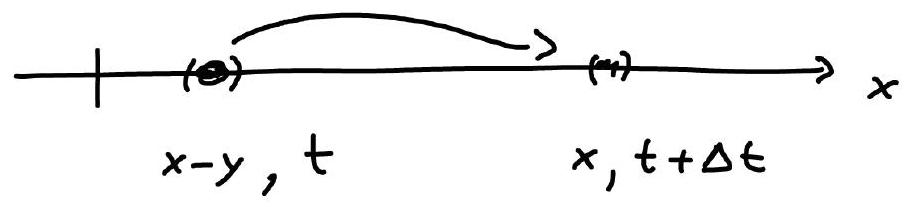
\includegraphics[width=\textwidth]{2025_10_26_8223bcdd8e86df21a973g-2}

The density of particles that we find at $x-y$ is $w(x-y, t)$ and each of these make a jump $y$ with prob. $f(y, \Delta t) d y$ in the following $\Delta t$. Thus the durity of particles at $x$, time $t+\Delta t$ is
\begin{DispWithArrows}[format=c, displaystyle]
w(x, t+\Delta t)=\int_{-\infty}^{+\infty} w(x-y, t) f(y, \Delta t) d y
\end{DispWithArrows}
We have assumed thot all perticles jump independently of each other. Further, we assume that that for suall st
\begin{enumerate}
  \item $f(y, \Delta t)$ decays fort with $y$ - jumps occur more likely clase to the initial point $x$
  \item $f(-y, \Delta t)=f(y, \Delta t)$ - jumps are qually likely from the left or from the right.
\end{enumerate}
With assumptions 1) and 2) we con Taylon expand w(+., ) in the integrand of $\varphi$. (9):
\begin{DispWithArrows}[format=c, displaystyle]
\int w(x-y, t) f(y, \Delta t) d y \simeq \int\left(w(x, t)-\left(\partial_{x} w\right) y+\frac{1}{2}\left(\partial_{x}^{2} w\right) y^{2}+\ldots\right) f(y, \Delta t) d y
\end{DispWithArrows}
Because $\int f(y, \Delta t) d y=1$
$\int w(x-y, t) f(y, \Delta t) d y \simeq w(x, t)+\frac{1}{2} \partial_{x}^{2} w \int_{-\infty}^{+\infty} y^{2} f(y, \Delta t) d y+h \circ t$ assume finite

We also write for small $\Delta t$ :
\begin{DispWithArrows}[format=c, displaystyle]
\int y^{2} f(y, \Delta t) d y=\frac{D \Delta t+h \circ t}{\int_{\text {as }} \Delta t \rightarrow 0}
\end{DispWithArrows}
then
\begin{DispWithArrows}[format=c, displaystyle]
w(x, t+\Delta t)=w(x, t)+\frac{1}{2} \Delta \Delta t \partial_{x}^{2} w+h \circ t
\end{DispWithArrows}
or
\begin{DispWithArrows}[format=c, displaystyle]
w \frac{(x, t+\Delta t)-w(x, t)}{\Delta t}=\frac{D}{2} \partial_{x}^{2} w+\sigma(\Delta t)
\end{DispWithArrows}
take the limit $\Delta t \rightarrow 0$
\begin{DispWithArrows}[format=c, displaystyle]
\frac{\partial w(x, t)}{\partial t}=\frac{D}{2} \partial_{x}^{2} w(x, t)
\end{DispWithArrows}
On d-dimensions :
\begin{DispWithArrows}[format=c, displaystyle]
\begin{aligned}
\frac{\partial w(F, t)}{\partial t}=\frac{D}{2} \nabla^{2} w(F, t) \\
\nabla^{2} \equiv \sum_{i}^{d} \frac{\partial^{2}}{\partial x_{i}^{2}}
\end{aligned}
\end{DispWithArrows}
Eq. (2) is the diffusion equation on heat equation. The PDE must be solved with an iritial condition $\left[
ight.$ e.g. $W(x, 0)=\delta\left(x-x_{0}\right)$ and, possibly, same boundery constitions.

\section*{Solution of the diffurion equation (scaling)}
Obsewetion: if $w(x, t)$ sobres $g$. (2) then so does $w\left(\lambda x, \lambda^{2} t\right)$ for any $\lambda \in \mathbb{R}(\lambda \neq 0)$ (try this out ) This scaling symmetry indicates that diffusion ef. has a dilation symmetry and $\frac{x^{2}}{t}$ is inversiant under suck scoling.

We make the assumption that such symmetry simplifies the form of the solution and this is only a function of $\frac{x}{\sqrt{D E}}$ (which is dimension less and preserves the symmety)
\begin{DispWithArrows}[format=c, displaystyle]
w(x, t)=u\left(\frac{x}{\sqrt{\Delta t}}\right) \quad u(z), z=\frac{x}{\sqrt{\Delta t}}
\end{DispWithArrows}
If we sub this into ep. (2) we get
\begin{DispWithArrows}[format=c, displaystyle]
\begin{gathered}
\partial_{t} w=\frac{d u}{d z} \frac{\partial z}{\partial t}=\frac{d u}{d z}\left(-\frac{x}{\sqrt{D}} \frac{1}{2} \frac{1}{t^{3 / 2}}\right) \\
\partial_{x}^{2} w=\partial_{x}\left(\frac{d u}{d z} \frac{\partial z}{\partial x}\right)=\frac{d^{2} u}{d z^{2}}\left(\frac{\partial z}{\partial x}\right)^{2}+\frac{d u}{d z} \frac{\partial^{2} z}{\partial x^{2}}=\frac{d^{2} u}{d z^{2}} \frac{1}{D t} \\
\partial_{t} w=-\frac{x}{2 \sqrt{D} t^{3 / 2}} \frac{d u}{d z}=\frac{D}{2} \underbrace{\frac{1}{d t} \frac{d^{2} u}{d z^{2}}}_{\partial_{x}^{2} w}=\frac{1}{2 t} \frac{d^{2} u}{d z}
\end{gathered}
\end{DispWithArrows}
We multiply both sides by $t$ :
\begin{DispWithArrows}[format=c, displaystyle]
-\underbrace{\frac{x}{\sqrt{D t}}} _{z} \frac{d u}{d z}=\frac{d^{2} u}{d z^{2}}
\end{DispWithArrows}
Finally
\begin{DispWithArrows}[format=c, displaystyle]
\frac{d^{2} u}{d z^{2}}+z \frac{d u}{d z}=0
\end{DispWithArrows}
which is an $O D E$ (no longer a $P D E$ ). Sefine $\rho=\frac{d u}{d z}$
\begin{DispWithArrows}[format=c, displaystyle]
\frac{d \rho}{d z}+z \rho=0 \quad \rightarrow \quad \rho(z)=a e^{-z^{2} / 2}
\end{DispWithArrows}
thus the final solution is $u(z)=a \int_{0}^{z} e^{-s^{2} / 2} d s+b$ where $a, b$ are detervined by initial conditions. The solution of ep. (2) is then
\begin{DispWithArrows}[format=c, displaystyle]
u\left(\frac{x}{\sqrt{\Delta t}}\right)=a \int_{0}^{\frac{x}{\sqrt{\Delta t}}} e^{-\frac{s^{2}}{2}} d s+b
\end{DispWithArrows}
$x>0, t \rightarrow \infty^{+} \quad u \longrightarrow a \int_{0}^{\infty} e^{-s^{2} / 2} d s+b=\sqrt{\frac{\pi}{2}} a+b$
\begin{DispWithArrows}[format=c, displaystyle]
x=0, t \neq 0 \quad u \longrightarrow b
\end{DispWithArrows}
This solution for general $a, b$ daes not satisfy the initial condition $w(x, 0)=\delta\left(x-x_{0}\right)$. Later on we will find the most general solution which sotisfies any initial condition.\\2) A more 
